\documentclass{article}

% Enforce utf-8 encoding-- only required if we're using the pdflatex engine.
% \usepackage[utf8]{inputenc}

% Packages for math
\usepackage{amsmath,amsfonts,amssymb,amsthm,epsfig,epstopdf,titling,url,array}

% Setup of thm env
\newtheorem{thm}{Theorem}

% Define norm display
\newcommand{\norm}[1]{\left\lVert #1 \right\rVert}

% Set double spacing 
\usepackage{setspace}
\doublespacing

% Drawing tools
\usepackage{tikz}
\usetikzlibrary{arrows}
\usetikzlibrary{fit}
\usetikzlibrary{positioning}

% Double figures
\usepackage{caption}
\usepackage{subcaption}

% Rotate text with \rotatebox{90}{Text}
\usepackage{graphicx}

% Parenthetical citations
\usepackage[round]{natbib} 

% Acronym definitions (ensures acronyms are always spelled out once)
\usepackage{acronym}
\acrodef{VaR}{Value at Risk}
\acrodef{dematel}[DEMATEL]{Decision-Making Trial and Evaluation Laboratory}

% Definition of Normal CDF function for plots.
\DeclareMathOperator{\CDF}{cdf}
\def\cdf(#1)(#2)(#3){0.5*(1+(erf((#1-#2)/(#3*sqrt(2)))))}%
\tikzset{
    declare function={
        normcdf(\x,\m,\s)=1/(1 + exp(-0.07056*((\x-\m)/\s)^3 - 1.5976*(\x-\m)/\s));
    }
}

% Title information
\author{AF/A9}
\title{The Air Force Comprehensive Core Capability Risk Assessment Framework}
\date{\today}

\begin{document}
\maketitle

\begin{abstract}
(To Complete Last)
\end{abstract}

\section{Introduction}
With an annual budget of over \$160 billion, operations on all seven continents, and more than 600,000 employees, the United States Air Force is one of the largest organizations in the world \citep{afbudget}. It is also among the most complex. While dropping bombs on an enemy target may be the most iconic Air Force mission, less than 1\% of all Air Force personnel find themselves performing that role. The remaining 99\% are responsible for the critical support infrastructure: the Air Force must recruit, educate, and train its own personnel; develop, procure, and sustain its aircraft; launch and operate its satellite constellations; and plan its operations in a way that supports national security objectives.

Figure \ref{fig:nss-network} illustrates these relationships. The United States seeks to ensure U.S. security, foster U.S. prosperity, promote universal values, and uphold the international order \citep{nss}. To support these objectives, the Pentagon publishes a list of high-level objectives for the Department of Defense, which the Air Force, along with the other services, must ensure they are capable of achieving. To communicate the capabilities that the Air Force provides the Department of Defense, the Air Force divides itself into a mutually exclusive and collectively exhaustive partition of \emph{core capabilities}. Although these core capabilities are themselves large aggregations, often with billions of dollars in annual budget, they can be thought of as distinct entities that influence each other and national military objectives. If there is risk in the Air Force core capabilities, then this risk will propagate to U.S. military objectives and ultimately hinder the U.S.' ability to achieve its security strategy.

\begin{figure}[!htb]
\centering
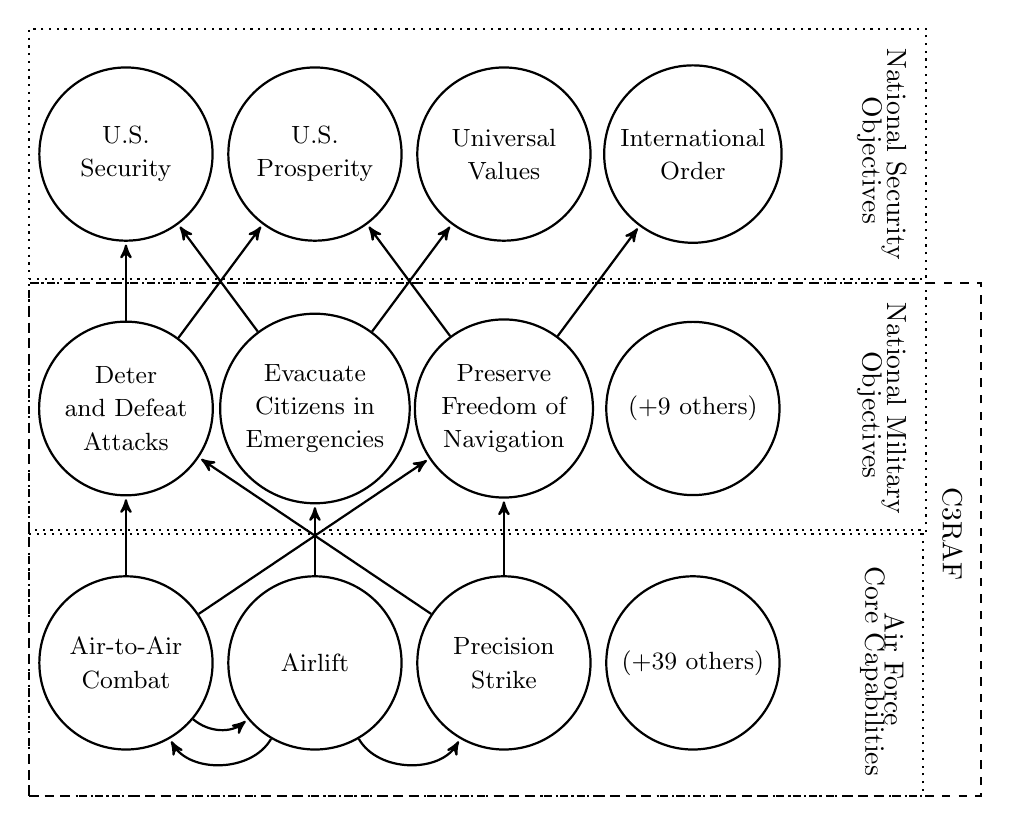
\begin{tikzpicture}[->,
                    >=stealth',
                    shorten >=1pt,
                    node distance=2.4cm,
                    thick,
                    nss/.style={circle,draw,minimum size=2.2cm},
                    %nms/.style={rectangle, draw, minimum width=2.2cm}
                    ]
% NSS
  \node[nss] (1) [align=center]{\small U.S. \\ \small Security};
  \node[nss] (2) [right of=1, align=center] {\small U.S. \\ \small Prosperity};
  \node[nss] (3) [right of=2, align=center] {\small Universal \\ \small Values};
  \node[nss] (4) [right of=3, align=center] {\small  International \\ \small Order};
  
  \node (5) [right of=4]{\rotatebox{270}{\hspace{5mm} Objectives}\rotatebox{270}{National Security}};
\node[draw,dotted,fit=(1) (2) (3) (4) (5)] {};

% NMS

\node[nss] (6) [below =1.0cm of 1, align=center]{\small Deter \\ \small and Defeat\\ \small Attacks};
\node[nss] (7) [right of=6, align=center]{\small Evacuate \\ \small Citizens in \\ \small  Emergencies};
\node[nss] (8) [right of=7, align=center]{\small Preserve \\ \small Freedom of\\ \small Navigation};
\node[nss] (9) [right of=8, align=center]{\small (+9 others)};

  \node (10) [right of=9]{\rotatebox{270}{\hspace{5mm} Objectives}\rotatebox{270}{National Military}};
\node[draw,dotted,fit=(6) (7) (8) (9) (10)] {};

\draw [->] (6) edge (1);
\draw [->] (6) edge (2);
\draw [->] (7) edge (1);
\draw [->] (7) edge (3);
\draw [->] (8) edge (2);
\draw [->] (8) edge (4);
% \draw [->] (9) edge (1); % this edge causes gross-looking overlap
%\draw [->] (9) edge (2);
%\draw [->] (9) edge (3);
%\draw [->] (9) edge (4);

\node[nss] (11) [below =1.0cm of 6, align=center]{\small Air-to-Air \\ \small Combat};
\node[nss] (12) [right of=11, align=center]{\small Airlift};
\node[nss] (13) [right of=12, align=center]{\small Precision \\ \small Strike} ;
\node[nss] (14) [right of=13, align=center]{\small (+39 others)};

  \node (15) [right of=14]{\rotatebox{270}{\hspace{1mm} Core Capabilities}\rotatebox{270}{\hspace{8mm}Air Force}};
\node[draw,dotted,fit=(11) (12) (13) (14) (15)] {};

\draw [->] (11) edge (6);
\draw [->] (11) edge (8);
\draw [->] (12) edge (7);
\draw [->] (13) edge (6);
\draw [->] (13) edge (8);
\draw [->] (12) edge[bend left=60] (11);
\draw [->] (12) edge[bend right=60] (13);
\draw [->] (11) edge[bend right=40] (12);

\node (16) [below right=-0.6cm and 0.2cm of 10]{\rotatebox{270}{\hspace{0mm}C3RAF}};
\node[draw,dashed,fit=(6) (16) (15) (10)] {};
\end{tikzpicture}
\caption{Relationships between Air Force core capabilities and National Security Strategy.}
\label{fig:nss-network}
\end{figure}

The scope, diversity, and uniqueness of the Air Force's core capabilities make enterprise risk management incredibly difficult. For these reasons, prior to this effort, Air Force risk management was largely confined to ``stove-pipes'' of operational chains-of-command. Although this arrangement is effective for a commander whose scope of authority is limited to a single core capability, those responsible for force integration cannot effectively compare risk across different core capabilities. Furthermore, interdependencies between Air Force core capabilities exacerbate this difficulty: even if you have a common risk ``currency'' across core capabilities, mitigating or accepting risk in one area may have higher order effects on others.

This paper develops a framework for addressing this challenge in integrating operational risk. First, we review applicable methods to compare risk across diverse operational settings and select an appropriate approach for a military context. Then, we develop a novel likelihood-maximization method for determining the interdependencies of the various Air Force core capabilities. We use these interdependencies to build a network model capable of integrating these risk assessments, producing a comprehensive estimate of Air Force effectiveness. Finally, we embed this network model in an optimization in order to determine the most effective portfolio of military risk. Although military classification prevents us from publishing our data or results, we illustrate our application of this methodology throughout with a representative example problem and discuss the publishable consequences of our analysis.

\section{Literature Review}
Three primary technical challenges exist to determine a comprehensive risk assessment:
\begin{enumerate}
\item How can we establish a common risk ``currency'' that allows commanders to compare risk in different core capabilities?
\item How can we quantitatively understand interdependencies between core capabilities?
\item How can we integrate these risk assessments and interdependencies?
\end{enumerate}
All three questions have literature precedent, which we now examine in turn.

\subsection{Risk Currency}
Like the Air Force, many public and private sector organizations face the problem of assessing risk across diverse operations. In the private sector, most risk is ultimately communicated in financial terms: how much can the company expect to lose? This intuition has led to a heavy reliance on financial-based risk metrics, such as \ac{VaR} \citep{jorion2000value, linsmeier2000value}. While metrics such as \ac{VaR} are useful when risk can be eliminated with an injection of funds, they are not directly applicable to military contexts. While a large bailout could immediately reduce a bank's financial risk to zero, a sudden injection of funds to the Air Force would not have any immediate effect on the Air Force's ability to strike targets in highly contested airspace.

Instead, military risk is typically assessed in terms of the probability of failing to meet mission objectives and the consequences of failing to do so \citep{joint-risk-manual}. Originally outlined in the 1980s \citep{kaplan}, practitioners have since applied this approach has extensively across a wide variety of military applications \citep{lincoln, monach, hamill,buckshaw,caswell2011analysis,kucik}.

Within the Air Force, operational risk is assessed through the Air Force Risk Assessment Framework \citep{gallagher2016improving}, which provides practical guidance for analysts. When applied to core capabilities, the framework prescribes the following:
\begin{enumerate}
\item Identify measurable metrics associated with the core capability.
\item Estimate a weight for each metric using a technique such as Value-Focused Thinking \citep{keeney2009value}. Weights should sum to 1. 
\item Estimate the probability of failure of each metric.
\item Summarize the core capability with the weighted sum of probability of failure.
\end{enumerate}

Often, the third step is the most challenging to accomplish in a defendable manner in a military context. For example, suppose we are trying to summarize the ``Airlift'' core capability, and we use the total weight of all materiel delivered as a metric.  We may know roughly how much materiel we can deliver, but the amount required is highly uncertain in the fog and friction of war \citep{clausewitz}. Due to the infrequency of armed conflicts, historic data is also unreliable or unavailable. Consequently, in most cases the demand distribution must be crafted manually by subject matter experts. 

Specifying a demand distribution manually is a fairly cognitively difficult task, especially for operational experts unfamiliar with probability distributions \citep{gallagher2016improving}. Consequently, most practitioners approximate the unknown demand distribution with a uniform distribution. Figure \ref{fig:airlift-risk} illustrates this approximation. 
\begin{figure}
\centering
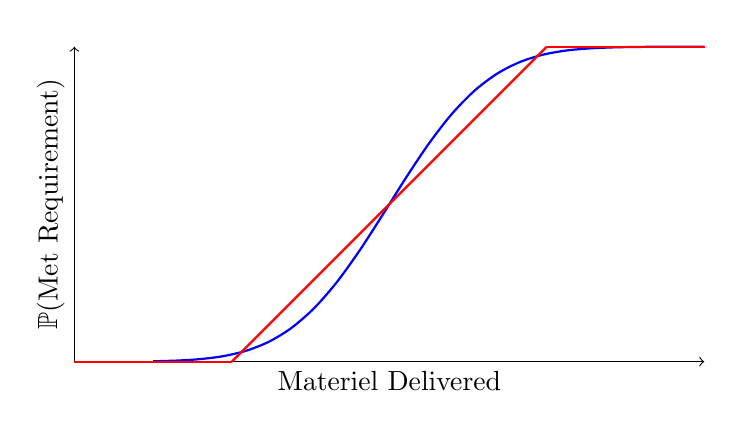
\begin{tikzpicture}
  \draw[->] (-0,0) -- (8,0) node[right] {};
  \draw[->] (0,0) -- (0,4) node[above] {};
  \draw[domain=0:7, smooth, variable=\x, blue, thick] plot({\x+1}, {4*normcdf(\x, 3, 1)});
  \draw[domain=0:2, smooth, variable=\x, red, thick] plot({\x}, {0});
  \draw[domain=2:6, smooth, variable=\x, red, thick] plot({\x}, {4/4*(\x-2)});
  \draw[domain=6:8, smooth, variable=\x, red, thick] plot({\x}, {4});
  \draw (4, 0) node[below] {Materiel Delivered};
  \draw (0, 2) node[left] {\rotatebox{90}{$\mathbb{P}(\text{Met Requirement})$}};
\end{tikzpicture}
\caption{Cumulative distribution function of required airlift (blue) and Air Force risk assessment framework approximation (red).}
\label{fig:airlift-risk}
\end{figure}
The simplicity of the uniform distribution allows for operational experts to easily define the distribution in terms of parameters with operational relevance: they simply specify the upper and lower bounds of what demand they believe to be plausible. This simplicity provides transparency and repeatability to the process, which is critical in the absence of objective data \citep{gallagher2016improving}.

\subsection{Determining Interdependencies}
Although mutually exclusive and collectively exhaustive, core capabilities often provide and receive support to one another. For example, before a fighter jet can engage targets, the pilot, support staff, munitions and fuel must be transported to the deployed airfield. Consequently, if there is risk in delivering the required support, then the effective risk of the core capability may be higher than initially reported. This phenomenon is exacerbated in cases of circular dependency, as shown in Figure \ref{fig:nss-network}: air-to-air combat capabilities must be present in order for supplies to be delivered by air, and supplies must be present in order to have air-to-air combat capabilities.

Ideally, we would measure these interdependencies directly. For example, if modeling different economic sectors, we could measure the amount of goods traded between industries \citep{leontief1986input}. However, in the military context, we lack a common measurable metric between core capabilities, and even if we had one, infrequency of military conflict prevents us from collecting representative data.

Lack of quantitative interdependency data is not a unique Air Force problem. \citet{dematel} developed a structured qualitative technique for assessing the relationships between complex systems, known as the \ac{dematel} method. This approach has been applied extensively across various domains \citep{dematel-overview}, such as supply chain design \citep{dematel-chiou}, environmental impact assessments \citep{dematel-green}, and marketing strategies \citep{dematel-chiu}.

The \ac{dematel} method consists of tasking experts to assess the first-order relationship between systems on a Likert scale \citep{likert}, and the averaging responses to assess the first-order dependence of system $i$ on system $j$, denoted $d_{ij}$. If we build a matrix of all such relationships, $[d_{ij}] = \mathbf{D}$, then we can calculate the infinite-order relationships $\mathbf{D}_\infty$ using the following: 
\begin{equation}
\begin{aligned}
\label{eqn:dematel}
\mathbf{D}_\infty & \triangleq \lim_{n \rightarrow \infty} \sum_{i=1}^n \mathbf{D}^i \\
& = \lim_{n \rightarrow \infty} (\mathbf{I}-\mathbf{D})^{-1}(\mathbf{I}-\mathbf{D})\sum_{i=1}^n \mathbf{D}^i \\
& = \lim_{n \rightarrow \infty} (\mathbf{I}-\mathbf{D})^{-1}(\mathbf{I}-\mathbf{D}^{n+1})\\
& = (\mathbf{I}-\mathbf{D})^{-1},
\end{aligned}
\end{equation}
where $\mathbf{I}$ is the appropriately-sized identity matrix and $\lim_{n\rightarrow \infty} \mathbf{D}^n=\mathbf{0}$ is ensured by normalizing $\mathbf{D}$ appropriately to ensure that its spectral radius is less than one \citep{dematel-overview}. Practitioners typically analyze the entries of $D_\infty$ directly for business insights \citep{dematel-overview, dematel-chiu, dematel-chiou}. 


\subsection{Integrating Risk and Interdependencies}
While the risk assessment framework of \citet{gallagher2016improving} provides a framework for assessing core capability risk and isolation, and the \ac{dematel} method provides a framework for assessing interdependencies between systems, we need an approach to synthesize the two pieces.

One approach to risk integration is the Leontief Inoperability Model \citep{haimes-iiom}. Originally proposed for infrastructure system, \citeauthor{haimes-iiom} model each system as a vertex in a network, and each first-order relationship a directed edge. When an individual system has some risk of inoperability, its risk propagates through the network until the network reaches some steady state. Mathematically, given a first-order dependency matrix $\mathbf{D}$, and initial risk $\mathbf{r}$, this model calculates the \emph{networked} risk to be 

\begin{equation}
\hat{\mathbf{r}} = \mathbf{r} + \mathbf{D} \hat{\mathbf{r}}
\end{equation}

Intuitively, this model takes the initial risk of each system and adds on the risk of all the systems upon which it depends. This model can also be written to solve for $\hat{\mathbf{r}}$ explicitly, i.e. 
\begin{equation}
\label{eqn:lin}
\hat{\mathbf{r}} = (\mathbf{I}-\mathbf{D})^{-1} \mathbf{r}.
\end{equation}
We also observe the similarity of this equation to the \ac{dematel} model: we can rewrite it as $\hat{\mathbf{r}} = \mathbf{D}_\infty \mathbf{r}$. This reformulation also gives insight into the nature of the model from the derivation of $\mathbf{D}_\infty$ in Equation \ref{eqn:dematel}, as it indicates that the inoperability model begins with the initial risk, then adds on the first-order risk inherited, then second order, and so forth.

The simplicity and effectiveness of the \citeauthor{haimes-iiom} model has led to its utilization in infrastructure development \citep{iiom-infrastructure}, hurricane cost estimation \citep{iiom-katrina}, and terrorism impact assessments \citep{iiom-terrorism}. 

\section{Methodology}

Literature precedent provides a solid foundation for us to build our comprehensive Air Force risk assessment. While the Risk Assessment framework of \citet{gallagher2016improving} is directly applicable, the \ac{dematel} and \citet{haimes-iiom} models must be modified to fit our application.

\subsection{Dependency Estimation}
The \ac{dematel} method assumes unbiased experts are available to determine the first-order relationships between systems $i$ and $j$ \citep{dematel-overview}. However, the Air Force does not have such experts in abundance: rather, expertise is generally acquired exclusively within the context of a single core capability. Consequently, while experts may be able to speak to dependencies and impacts of their core capabilities, they did not feel comfortable assessing other relationships. Parochialism adds another layer of complexity: in the author's experience, experts tend to overestimate the usefulness of their core capability to others while underestimating the magnitude of support it requires.

Imposing additional structure on the responses of the experts can help alleviate these problems \citep{ahp}. One approach could be to constrain the number of times an expert gives a minimal or maximum assessment of a dependency. However, without prior knowledge of the structure of the network, this constraint would be entirely arbitrary. 

An alternative approach could exploit the fact that our experts only feel comfortable assessing relationships directly tied to their assigned core capability. Instead of instructing experts to assess each relationship individually, we could give each core capability expert 100 ``points,'' which he or she could proportionally allocate to the other core capabilities that the expert's core capability depends on. Similarly, each core capability expert could get 100 ``points'' to allocate to the core capabilities that the expert's core capability provides support to. 

Figures \ref{fig:point} illustrate this constraint through the lens of an expert on air to air combat. In Figure \ref{fig:point-dep}, the expert acknowledges that air to air combat is heavily dependent on the capability of suppressing enemy air defenses, and allocates 50 of her 100 points to that core capability. Air refueling and pilot training are also important, but less so, so she awards them 20 points each. Precision strikes are rarely required to support air to air combat, so the remaining ten points are allocated to that capability. The expert similarly assesses the relative impacts of air to air combat on those core capabilities, as illustrated in Figure \ref{fig:point-imp}. 
\begin{figure}[!htb]
\centering
\begin{subfigure}{.5\textwidth}
\centering
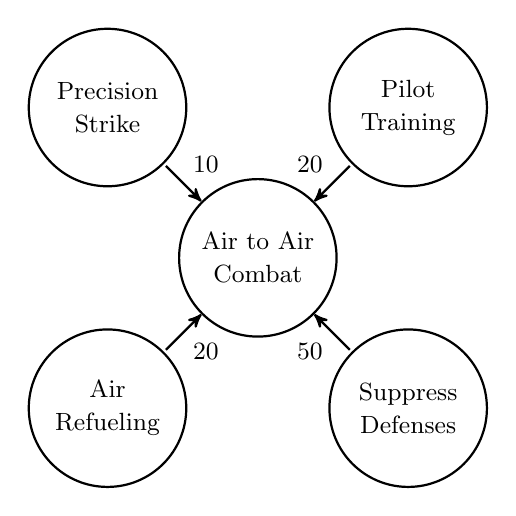
\begin{tikzpicture}[->,
                    >=stealth',
                    shorten >=1pt,
                    node distance=2.7cm,
                    thick,
                    nss/.style={circle,draw,minimum size=2.0cm}
                    %nms/.style={rectangle, draw, minimum width=2.2cm}
                    ]
  \node[nss] (1) [align=center]{\small Air to Air \\ \small Combat};
  \node[nss] (2) [below right of=1, align=center]{\small Suppress\\ \small Defenses};
  \node[nss] (3) [below left  of=1, align=center]{\small Air\\ \small Refueling};
  \node[nss] (4) [above left  of=1, align=center]{\small Precision\\ \small Strike};
  \node[nss] (5) [above right of=1, align=center]{\small Pilot\\ \small Training};
  \draw [<-] (1) edge node[below left]  {\small 50} (2);
  \draw [<-] (1) edge node[below right] {\small 20} (3);
  \draw [<-] (1) edge node[above right]  {\small 10} (4);
  \draw [<-] (1) edge node[above left] {\small 20} (5);
\end{tikzpicture}
\caption{Prioritized dependencies.}
\label{fig:point-dep}
\end{subfigure}%
\begin{subfigure}{0.5\textwidth}
\centering
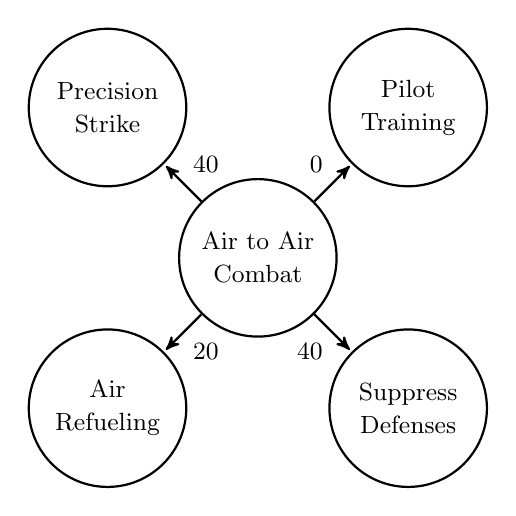
\begin{tikzpicture}[->,
                    >=stealth',
                    shorten >=1pt,
                    node distance=2.7cm,
                    thick,
                    nss/.style={circle,draw,minimum size=2.0cm}
                    %nms/.style={rectangle, draw, minimum width=2.2cm}
                    ]
  \node[nss] (1) [align=center]{\small Air to Air \\ \small Combat};
  \node[nss] (2) [below right of=1, align=center]{\small Suppress\\ \small Defenses};
  \node[nss] (3) [below left  of=1, align=center]{\small Air\\ \small Refueling};
  \node[nss] (4) [above left  of=1, align=center]{\small Precision\\ \small Strike};
  \node[nss] (5) [above right of=1, align=center]{\small Pilot\\ \small Training};
  \draw [->] (1) edge node[below left]  {\small 40} (2);
  \draw [->] (1) edge node[below right] {\small 20} (3);
  \draw [->] (1) edge node[above right]  {\small 40} (4);
  \draw [->] (1) edge node[above left] {\small 0} (5);
\end{tikzpicture}
\caption{Prioritized impacts.}
\label{fig:point-imp}
\end{subfigure}
\caption{Notional assessment of air-to-air combat relationships to other capabilities.}
\label{fig:point}
\end{figure}

Although imposing this structure on the experts does increase the repeatability of the elicitation, it does add a layer of complexity, as the points the experts allocated are only meaningful in relative terms. For example, while Figure \ref{fig:point-dep} indicates that the expert believes air to air combat requires air refueling twice as much as it requires precision strike, it does not provide an estimate for what percentage of missions require air refueling. Similarly, the air refueling expert may allocate 30 impact points to air-to-air combat, but these 30 points only have intrinsic meaning relative to the other capabilities air refueling impacts. Although both estimates of the same relationship|the dependence of air to air combat on air refueling|the two assessments not directly comparable.

In order to combine the two assessments, we apply a maximum-likelihood estimation technique \citep{mle}. Suppose $\mathbf{D}_D$ is the ``dependency'' matrix, where each entry $d_{ij}^{(D)}$ contains the dependency points expert $i$ allocated to core capability $j$. Conversely, let $\mathbf{D}_I$ be the ``impact'' matrix where each element $d_{ij}^{(D)}$ is number of impact points core capability $j$ allocated to core capability $i$. Due to our constraint that experts can only allocate 100 impact points and 100 dependency points, we know that the rows of $\mathbf{D}_D$ must sum to 100, and the columns of $\mathbf{D}_I$ must sum to 100.

Now, suppose $\widehat{\mathbf{D}}$ is an arbitrary guess for the true relationship matrix $\mathbf{D}$. If this guess were correct, then we would expect that the experts would have assessed dependency matrix $\widehat{\mathbf{D}_D}$, where we model the forced prioritization of the experts by dividing each element of $\widehat{\mathbf{D}}$ by its row sum, and then multiplying by 100. Similarly, if $\widehat{\mathbf{D}}$ were the correct relationship matrix, then we can calculate the impact matrix the experts would have assessed, $\widehat{\mathbf{D}_I}$, by dividing each element of $\widehat{\mathbf{D}}$ by its column sum and multiplying by 100.

In other words, we would have expected to see matrices $\widehat{\mathbf{D}_I}$ and $\widehat{\mathbf{D}_D}$, but instead, our data were $\mathbf{D}_D$ and $\mathbf{D}_I$. By assuming normally distributed error, we can calculate the likelihood of our guess $\widehat{\mathbf{D}}$ using the Frobenious norm:

\begin{equation}
\label{eqn:likelihood}
\mathbb{P}\left(\mathbf{D}_I, \mathbf{D}_D \mid \widehat{\mathbf{D}}\right) \propto \norm{\mathbf{D}_D - \widehat{\mathbf{D}_D }}_\mathcal{F}^2 + \norm{\mathbf{D}_I - \widehat{\mathbf{D}_I }}_\mathcal{F}^2
\end{equation}

By finding the value of $\widehat{\mathbf{D}}$ that maximizes Equation \ref{eqn:likelihood}, we can estimate the true value of the underlying relationships. Although the normalization of $\widehat{\mathbf{D}}$ to create $\widehat{\mathbf{D}_D}$ and $\widehat{\mathbf{D}_I}$ makes this optimization nonconvex, heuristic searches such as the Nelder-Mead method \citep{nelder1965simplex} can still identify a reasonable estimate for $\widehat{\mathbf{D}}$.

Another significant drawback of this normalization is that the value of Equation \ref{eqn:likelihood} is identical for all matrices that are scalar multiples. Consequently, once the optimization algorithm converges to a $\widehat{\mathbf{D}}$, we must identify the scalar multiple of that matrix to use in the risk propagation model. We describe the method used to determine this scalar in Section \ref{section:application}. 

\subsection{Risk Propagation}

While the \citeauthor{haimes-iiom} model is generally useful, it poses several problems when applied to studying military risk. First, its additive definition does not constrain the elements of $\hat{\mathbf{r}}$ to be in $[0,1]$. Although its output may still be useful, estimates of ``110\%'' probability of inoperability undermine the model's credibility when presenting to decision makers. 

A more serious concern is the constraint that the spectral radius of $\mathbf{D}$ be less than 1. For example, in a military context, the following network may in fact exist:

\begin{figure}[!htb]
\centering
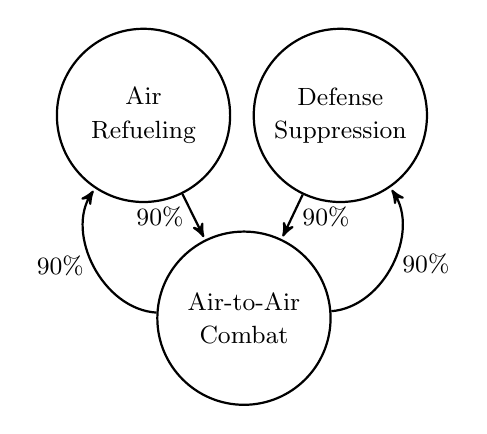
\begin{tikzpicture}[->,
                    >=stealth',
                    shorten >=1pt,
                    node distance=2.5cm,
                    thick,
                    nss/.style={circle,draw,minimum size=2.2cm},
                    %nms/.style={rectangle, draw, minimum width=2.2cm}
                    ]
  \node[nss] (1) [align=center]{\small Air \\ \small Refueling};
  \node[nss] (2) [right of=1, align=center]{\small Defense\\ \small Suppression};
  \node[nss] (3) [below right=1cm and -0.3cm of 1, align=center]{\small Air-to-Air\\ \small Combat};
  \draw [->] (1) edge node[left] {\small 90\%} (3);
  \draw [->] (2) edge node[right] {\small 90\%} (3);
  \draw [->] (3) edge[bend left=60] node[left] {\small 90\%} (1);
  \draw [->] (3) edge[bend right=60] node[right] {\small 90\%} (2);
\end{tikzpicture}
\caption{Network for which the spectral radius of the relationship matrix $\mathbf{D}$ exceeds one.}
\label{fig:ovary}
\end{figure}
The $\mathbf{D}$ matrix for Figure \ref{fig:ovary} is 
\begin{equation*}
\mathbf{D} = 
\begin{bmatrix}
0 & 0 & 0.9 \\
0 & 0 & 0.9 \\
0.9 & 0.9 & 0\\
\end{bmatrix},
\end{equation*}
which has a spectral radius of 1.3. Consequently, the assumption in the \ac{dematel} method that $\lim_{n\rightarrow \infty} \mathbf{D}^n = \mathbf{0}$ does not hold, and attempts to apply Equation \ref{eqn:lin} result in the counterintuitive property that increases in risk may decrease the risk of the dependent capabilities. While normalizing $\mathbf{D}$ would alleviate this problem, the normalized $\mathbf{D}$ would no longer reflect the underlying reality. 

An alternative formulation to risk propagation could be to use elementary probability rules. Suppose core capability $i$ depends on core capability $j$ 50\% of the time, and suppose core capabilities $i$ and $j$ have a risk of 30\% and 40\% of failing independently. Then, we would expect that the true risk of core capability $i$, denoted $\hat{r_i}$, is 

\begin{equation}
\label{prob-example}
\hat{r_i} = (1-0.3)(1-0.5\cdot 0.4)
\end{equation}

If we let $r_i$ denote the risk of each core capability failing independently, then we can extend this intuition to relate a core capability to an arbitrary number of dependencies:

\begin{equation}
\label{eqn:rel}
1-\hat{r_i} = (1-r_i)\prod_j  \left(1-d_{ij}\hat{r_j}\right),
\end{equation}

Although intuitive, this formulation is recursively defined, and its solution cannot be determined algebraically. However, we can solve it iteratively:

\begin{equation}
\mathbf{\hat{r}}^{(i+1)} = f\left(\mathbf{\hat{r}}^{(i)}\right) = \begin{bmatrix} 
1-(1-r_1)\prod_j  (1-d_{1j}\hat{r_j}^{(i)}\\
\vdots\\
1-(1-r_n)\prod_j  (1-d_{nj}\hat{r_j}^{(i)}).
\end{bmatrix}
\end{equation}

Convergence of this fixed-point iteration is guaranteed as a consequence of Theorem \ref{thm:lipschitz} \citep{linear-algebra}. 

\begin{thm}
\label{thm:lipschitz}
The function $f$ described in Equation \ref{eqn:rel} is locally Lipschitz continuous in the set $r_i, d_{ij} \in [0,1] \hspace{1mm} \forall \hspace{1mm} i,j$.
\end{thm}
\begin{proof}
We proceed directly and show that Lipschitz continuity holds for each element $\hat{r_i}$. Let $\mathbf{x}^{(1)}$ and $\mathbf{x}^{(2)}$ be arbitrary elements of $[0,1]^n$ and let $i$ be an arbitrary index between 1 and $n$. Then, 

\begin{equation}
f\left(\mathbf{x}^{(1)}\right) - f\left(\mathbf{x}^{(2)}\right) = 
\begin{bmatrix}
\vdots \\
(1-r_i)\left( \prod_j \left(1-d_{ij} x_j^{(1)} \right) -  \prod_j \left(1-d_{ij} x_j^{(2)} \right) \right)\\
\vdots\\
\end{bmatrix}
\end{equation}
Because $d_{ij}\in [0,1]$ and $x_{j}\in [0,1]$, we note that the maximum value of $\prod_j \left(1-d_{ij} x_j^{(1)} \right) -  \prod_j \left(1-d_{ij} x_j^{(2)} \right)$ is $x_i^{(1)} - x_j^{(2)}$. Consequently, $(1-r_i)$ is our Lipschitz constant and we have Lipschitz continuity along each dimension, which is sufficient for Lipschitz continuity in $\mathbb{R}^n$.
\end{proof}

While this approach initially seems unrelated to the \citeauthor{haimes-iiom} model, the two share a fundemental relationship described in Theorem \ref{thm:first-order}. 
\begin{thm}
\label{thm:first-order}
The \citeauthor{haimes-iiom} model is a first-order approximation of Equation \ref{eqn:rel}.
\end{thm}
\begin{proof}
We begin by taking the natural logarithm of both sides of Equation \ref{eqn:rel} and applying the identity $\log(ab) = \log(a) + \log(b)$. This substitution yields

\begin{equation}
\log(1-\hat{r_i}) = \log(1-r_i) + \sum_j \log( 1-d_{ij}\hat{r_j}).
\end{equation}

We now apply the first order Taylor series of $\log(x)$ about $x=1$, namely $\log(x) = -1 + x + \mathcal{O}\left(x^2\right)$,

\begin{equation}
\label{eqn:approx}
\hat{r_i} + \mathcal{O}(\hat{r_i}^2) = {r_i} + \mathcal{O}\left({r_i}^2\right) + \sum_j \left(d_{ij}\hat{r_j} + \mathcal{O}\left((\hat{r_j})^2 \right)\right).
\end{equation}
By dropping the big-$\mathcal{O}$ terms in Equation \ref{eqn:approx} and writing the system in matrix form, we recover the linear formulation in Equation \ref{eqn:lin}.
\end{proof}

We could also model the risk propagation using a third formulation that assumes dynamic re-prioritization of capabilities within the Air Force. The relationship
\begin{equation}
\label{eqn:max}
\hat{r_i} = \max_j \left(r_i, d_{ij}\hat{r_j}\right)
\end{equation}
codifies this belief, as it indicates that the capabilities of the Air Force intelligently align themselves to ensure overlap of their successes. 

If we let $\hat{r}_i^L$ denote the estimate for $\hat{r_i}$ using Equation \ref{eqn:lin},  $\hat{r}_i^P$ denote the estimate of $\hat{r_i}$ produced using Equation \ref{eqn:rel}, and $\hat{r}_i^M$ denote the estimate of $\hat{r_i}$ produced using Equation \ref{eqn:max}, then Theorem \ref{thm:bounds} establishes a fundamental relationship between their outputs.

\begin{thm}
\label{thm:bounds}
For all $i$, $\hat{r}_i^M \leq \hat{r}_i^P \leq \hat{r}_i^L$. 
\end{thm}
\begin{proof}

We first show that $\hat{r}_i^L \geq \hat{r}_i^P$. We proceed by induction on the number of elements for which $d_{ij}$ is nonzero.

\emph{Base Step.} If $d_{ij}=0 \hspace{1mm} \forall \hspace{1mm} i,j$, then Equations \ref{eqn:rel} and \ref{eqn:lin} are identical, indicating that $\hat{r}_i^L = \hat{r}_i^P$. 

\emph{Inductive Step.} Suppose $\hat{r}_i^L \geq \hat{r}_i^P$ holds for $n$ nonzero $d_{ij}$ elements, and we discover an additional nonzero $d_{ij}$ relationship. Then, by Equation \ref{eqn:lin} the value of $1-\hat{r}_i^L$ will decrease by $d_{ij}\hat{r_j}$, but the change in $\hat{r}_i^P$ will be $\hat{r}_i^P - \hat{r}_i^P(1-d_{ij}\hat{r_j}) = \hat{r}_i^P d_{ij}\hat{r_j}$ by Equation \ref{eqn:rel}. Because $0 \leq \hat{r}_i^P \leq 1$, we have that the increase in $\hat{r}_i^L$ must be greater than the increase in $\hat{r}_i^P$. Thus, $\hat{r}_i^L \geq \hat{r}_i^P$ must also hold for $n+1$ nonzero $d_{ij}$ elements, completing our induction.

Now, we establish that $\hat{r}_i^P \geq \hat{r}_i^M$. We again proceed by induction on the number of elements for which $d_{ij}$ is nonzero.

\emph{Base Step.} If $d_{ij}=0 \hspace{1mm} \forall \hspace{1mm} i,j$, then Equations \ref{eqn:rel} and \ref{eqn:max} are identical, indicating that $\hat{r}_i^M = \hat{r}_i^P$. 

\emph{Inductive Step.} Suppose $\hat{r}_i^P \geq \hat{r}_i^M$ holds for $n$ nonzero $d_{ij}$ elements, and we discover an additional nonzero $d_{ij}$ relationship. Then, by Equation \ref{eqn:max} the value of $1-\hat{r}_i^M$ will be $\min\left(1-\hat{r_i}, 1-d_{ij}\hat{r_j}\right)$, while by Equation \ref{eqn:rel} the value of $1-\hat{r}_i^P$ will be $(1-\hat{r_i})(1-d_{ij}\hat{r_j})$. Because both $(1-\hat{r_i})$ and $(1-d_{ij}\hat{r_j})$ are in the range $[0,1]$, we know that $(1-\hat{r_i})(1-d_{ij}\hat{r_j}) \leq \min\left(1-\hat{r_i}, 1-d_{ij}\hat{r_j}\right)$, which indicates that $\hat{r}_i^P \geq \hat{r}_i^M$ and completes our induction.
\end{proof}

Theorem \ref{thm:bounds} is a powerful result that bounds the nonlinear behavior of Equation \ref{eqn:rel} by the linear behavior of Equations \ref{eqn:lin} and \ref{eqn:max}. While the nonlinear probability model must be solved iteratively, its output can be bounded through deterministic calculations. Furthermore, if we wished to explore variations on $\mathbf{r}$, e.g. to find one that minimizes network risk, we could explore the linear upper and lower bounds in polynomial time by using linear programming \citep{lp}.

\section{Application}
\label{section:application}

\section{Conclusion}

\bibliographystyle{plainnat}
\bibliography{sources}

\end{document}
